\chapter{Arhitectura aplicației}

\section{Microservicii}

Microserviciile sunt o arhitectură care presupune segmentarea unei aplicații într-o suită de servicii specializate, independente, ce comunică prin protocoale light-weight, în mod popular transmițând date prin HTTP într-un context RESTful. Unul din avantajele principale ale acestei arhitecturi este decuplarea serviciilor implicate. Eșecul unui serviciu nu afectează întreaga aplicație, astfel încât problemele se manifestă izolat și sunt mai ușor de controlat. Un alt motiv pentru care am considerat că această arhitectură este potrivită aplicației este versatilitatea permisă în alegerea tehnologiilor și a limbajelor de programare. 

 \begin{figure}[ht]
	\centering
 	 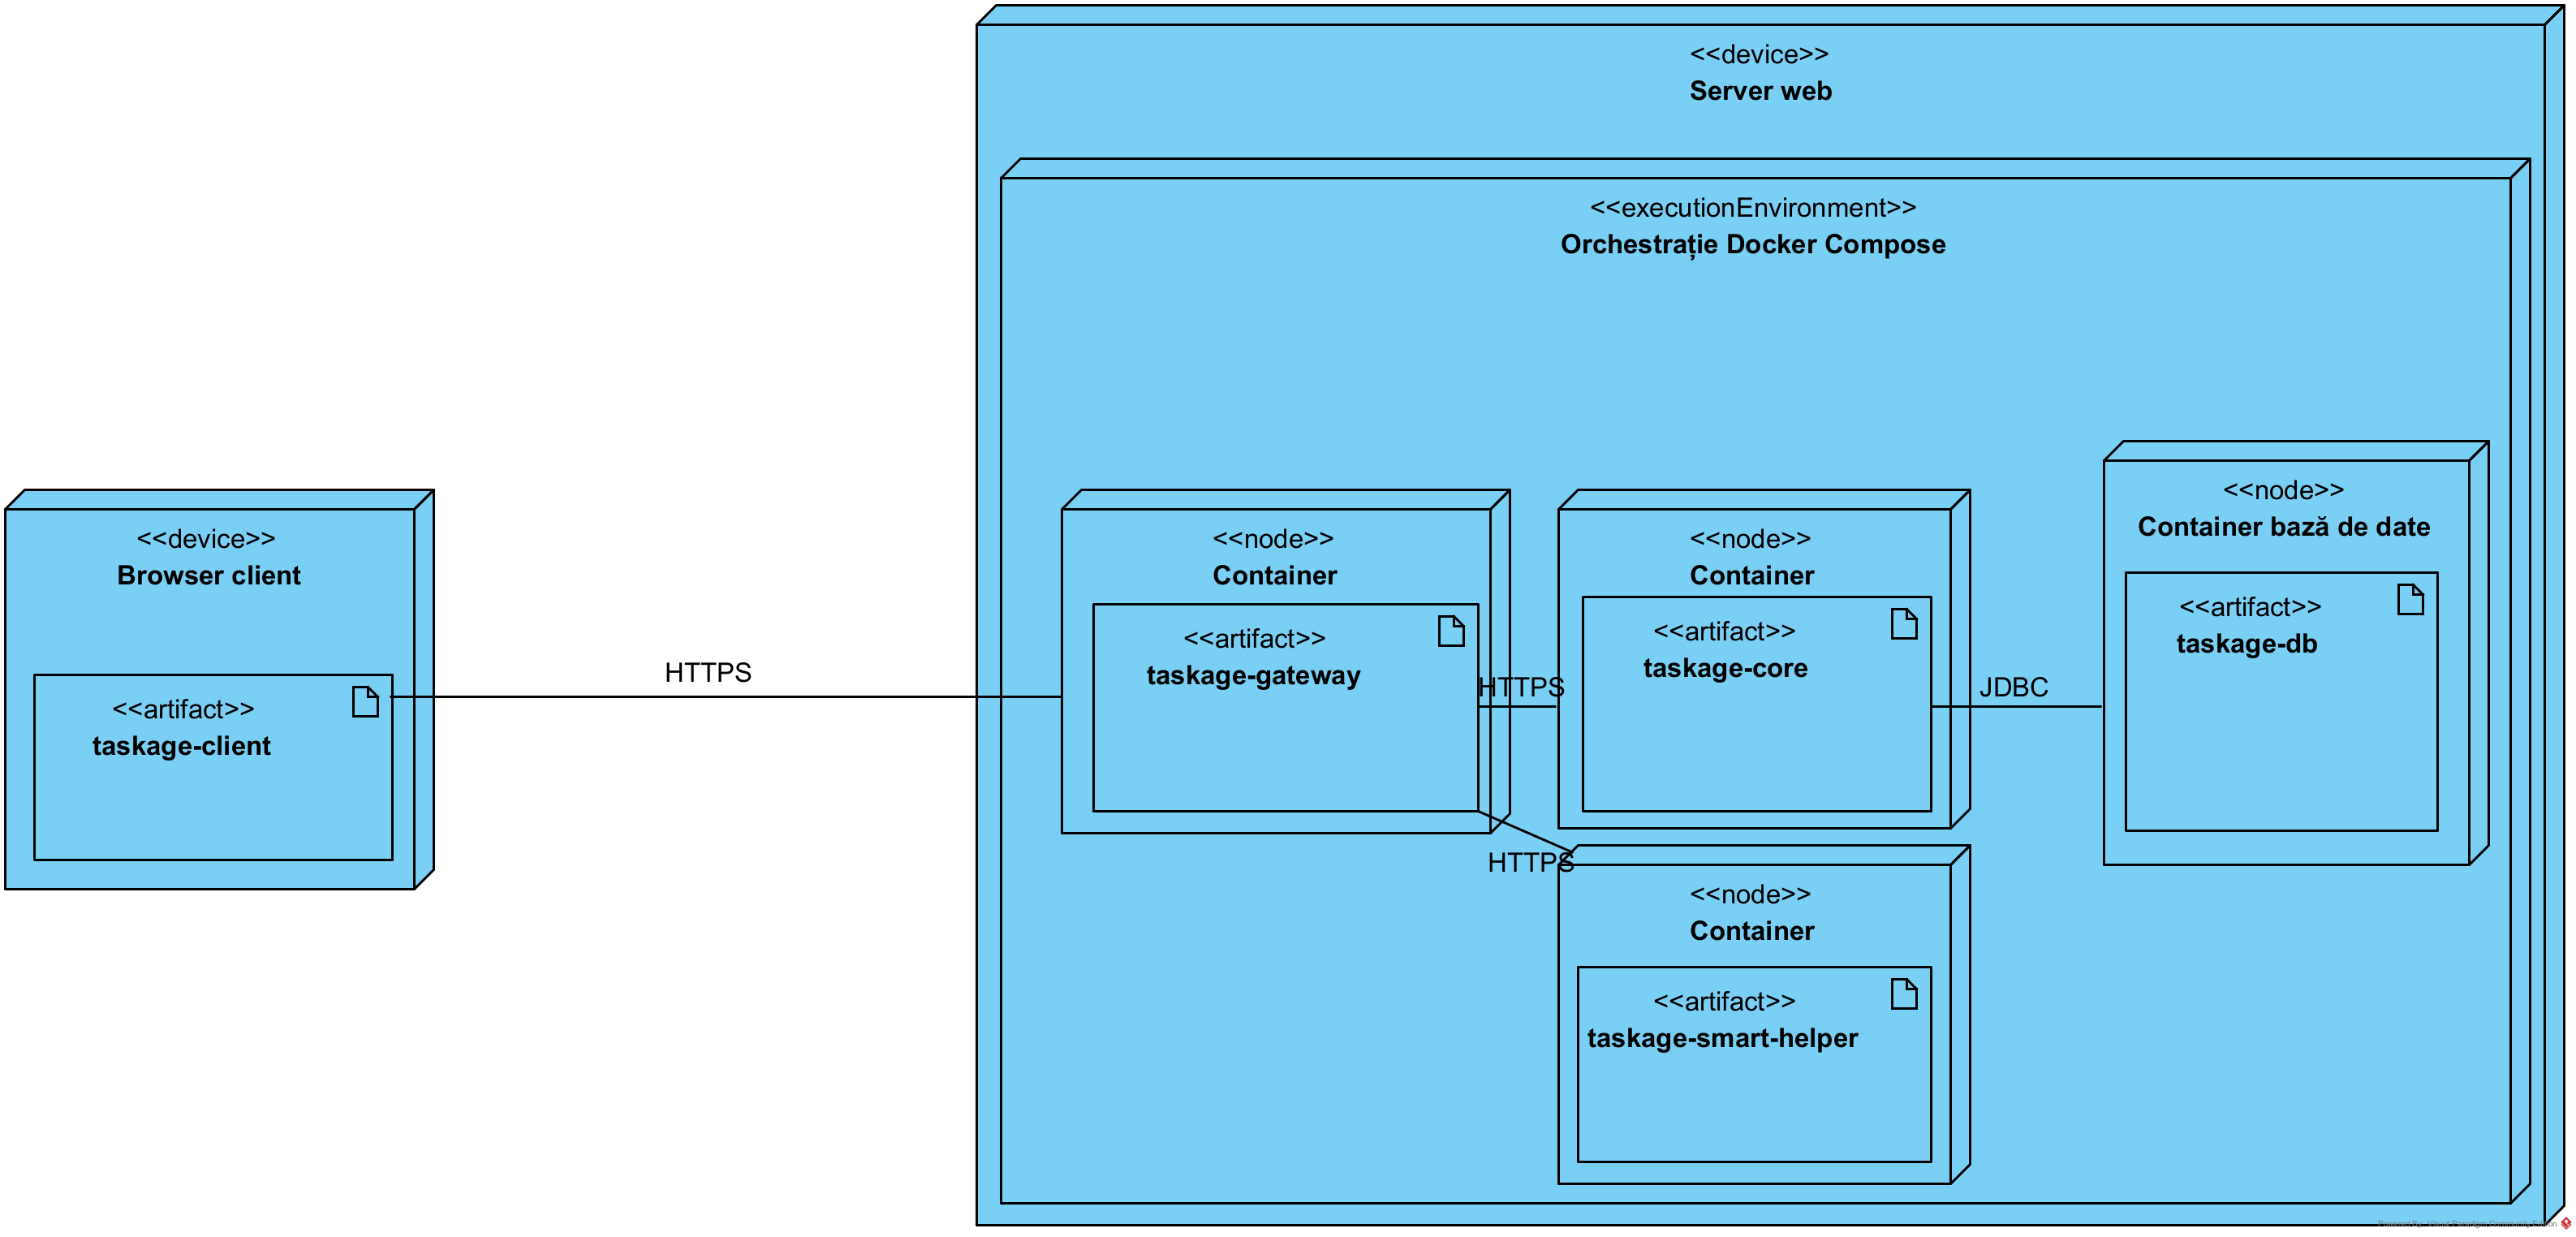
\includegraphics[width=\linewidth]{deployment-diagram-1.png}
	\caption{Arhitectura high-level}
	\label{fig:deployment-diagram-1}
 \end{figure}

Figura 3.1 ilustrează caracteristica modulară a aplicației. Pe partea de front-end, artefactul aplicației React taskage-client rulează în browser-ul web al utilizatorului prin codul transpilat din TSX în JS. Acesta comunică cu serverul prin apeluri HTTP, utilizând componenta Spring Cloud taskage-gateway ca punct de intrare către functionalitățile back-end. Serviciile de back-end comunică la rândul lor prin protocolul HTTP, iar conexiunea la baza de date este facilitată de JDBC.

[de completat legaturile taskage-smart-helper cu bd dupa ce ma hotarasc daca fac alt db sau continui pe acelasi]

\section{taskage-core}

 \begin{figure}[ht]
	\centering
 	 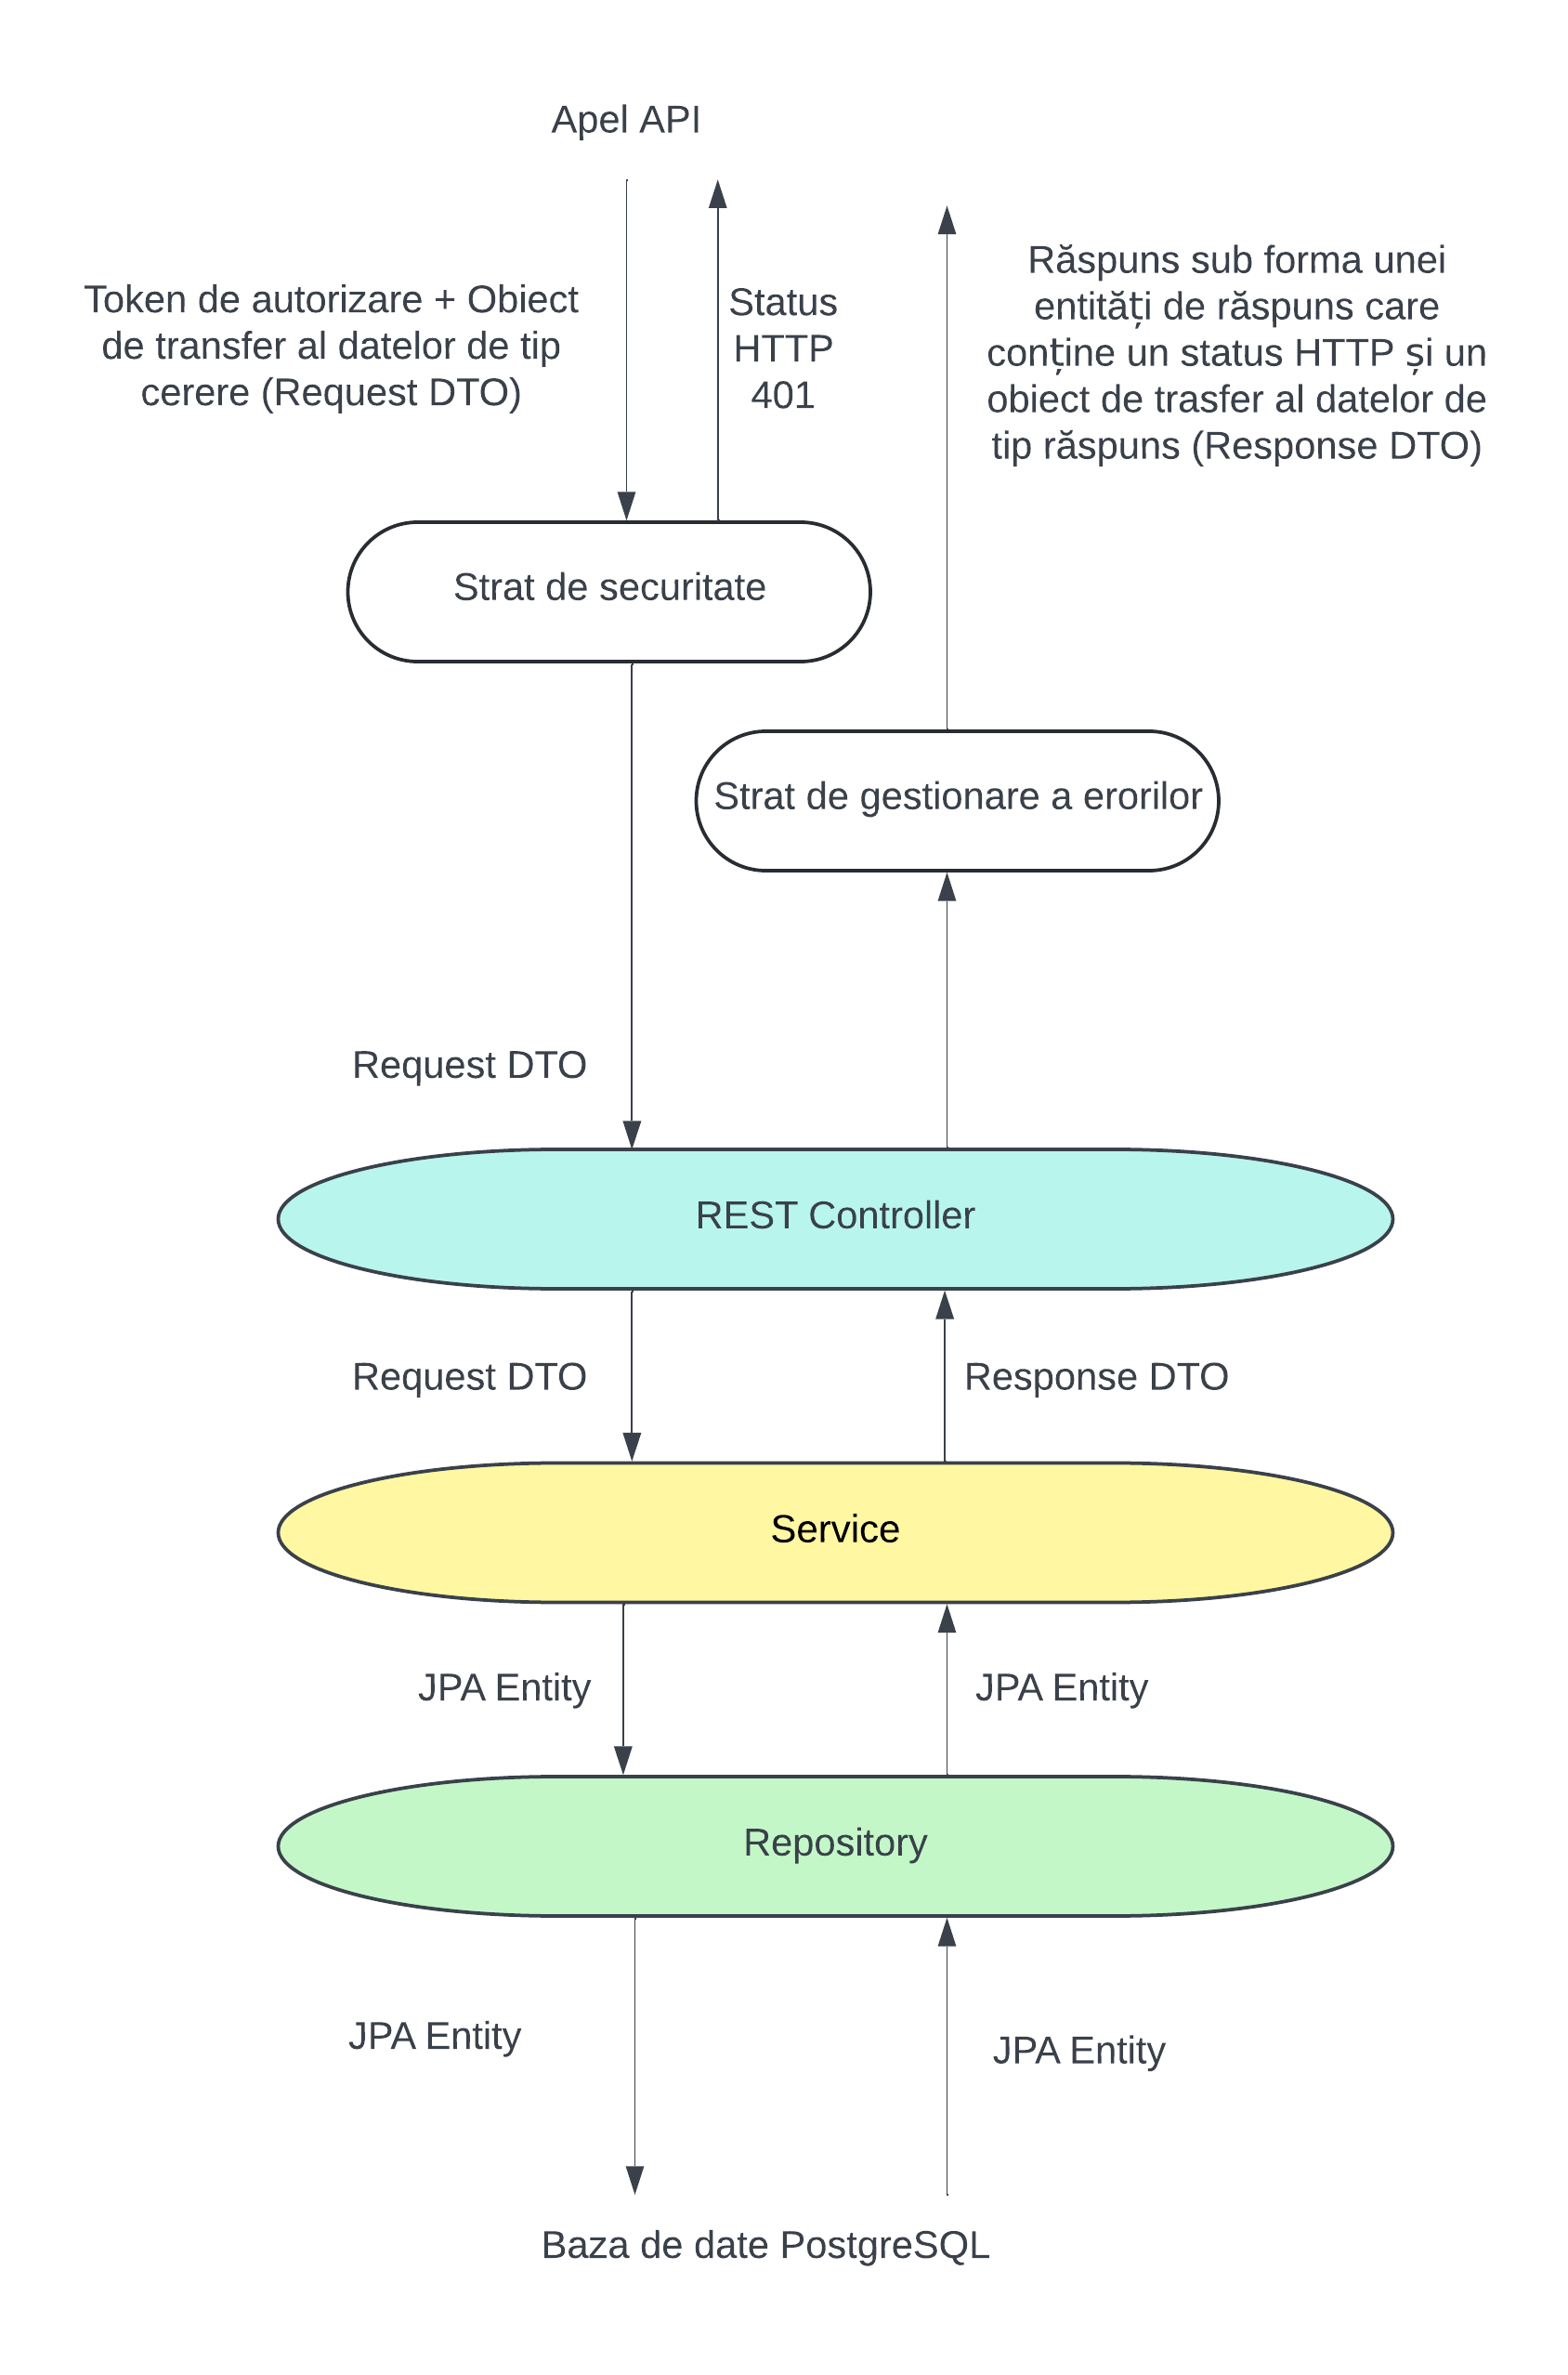
\includegraphics[width=0.6\linewidth]{controller-service-repository-flow.png}
	\caption{Fluxul datelor în componenta core}
	\label{controller-service-repository-flow}
 \end{figure}

Componenta care se ocupă cu funcționalitățile cele mai de bază ale aplicației este taskage-core. Aici se realizează operațiile CRUD asupra entităților și se gestionează cererile uzuale ale platformei. Structura componentei urmează patternul Controller-Service-Repository, popular în aplicațiile Spring Boot. Acest model de structurare a proiectului urmărește separarea sarcinilor unui sistem mare în părți mai ușor de manevrat. Fluxul datelor, reprezentat în figura 3.2, este controlat, iar fiecare strat are un scop bine definit. 

Apelurile HTTP conțin un JWT token în header și trec prin filtrul de autorizare, implementat cu ajutorul Spring Securit. Dacă tokenul este aprobat ca fiind valabil și având criptat rolul corespunzător, apelul ajunge la end-point-ul asociat din controller. Altfel, aplicația intoarce un răspuns cu status HTTP 401(Unauthorized). Controllerele constituie API-ul aplicației și ca au ca unic scop expunerea unor funcționalități către agenți externi. Datele sunt primite sub forma unui obiect de transfer al datelor(Request DTO), care nu se traduce într-o entitate a bazei de date, fiind doar un mod de transmitere a informației între microservicii. Aceste DTO-uri trebuie de asemenea să respecte validările impuse câmpurilor prin Jakarta Validation.

Dacă DTO-ul a fost validat, acesta este trimis mai departe pentru procesare în zona cu logica de afaceri a aplicației, și anume serviciile. Serviciile procesează informația și eventual o mapează ca entități JPA spre a o transmite mai departe depozitelor(repositories). Depozitele reprezintă stratul de acces al datelor și se ocupă cu toate interacțiunile cu baza de date. Dacă totul se realizează cu succes, se va returna o entitate de răspuns cu statusul HTTP 200, eventual conținând un Response DTO cu datele cerute. Dacă se aruncă vreo excepție, aceasta va fi prinsă de clasa care se ocupă cu gestiunea erorilor la nivel global, GlobalExceptionHandler, și se va trimite înapoi un răspuns sugestiv.

\section{taskage-db}

 \begin{figure}[ht]
	\centering
 	 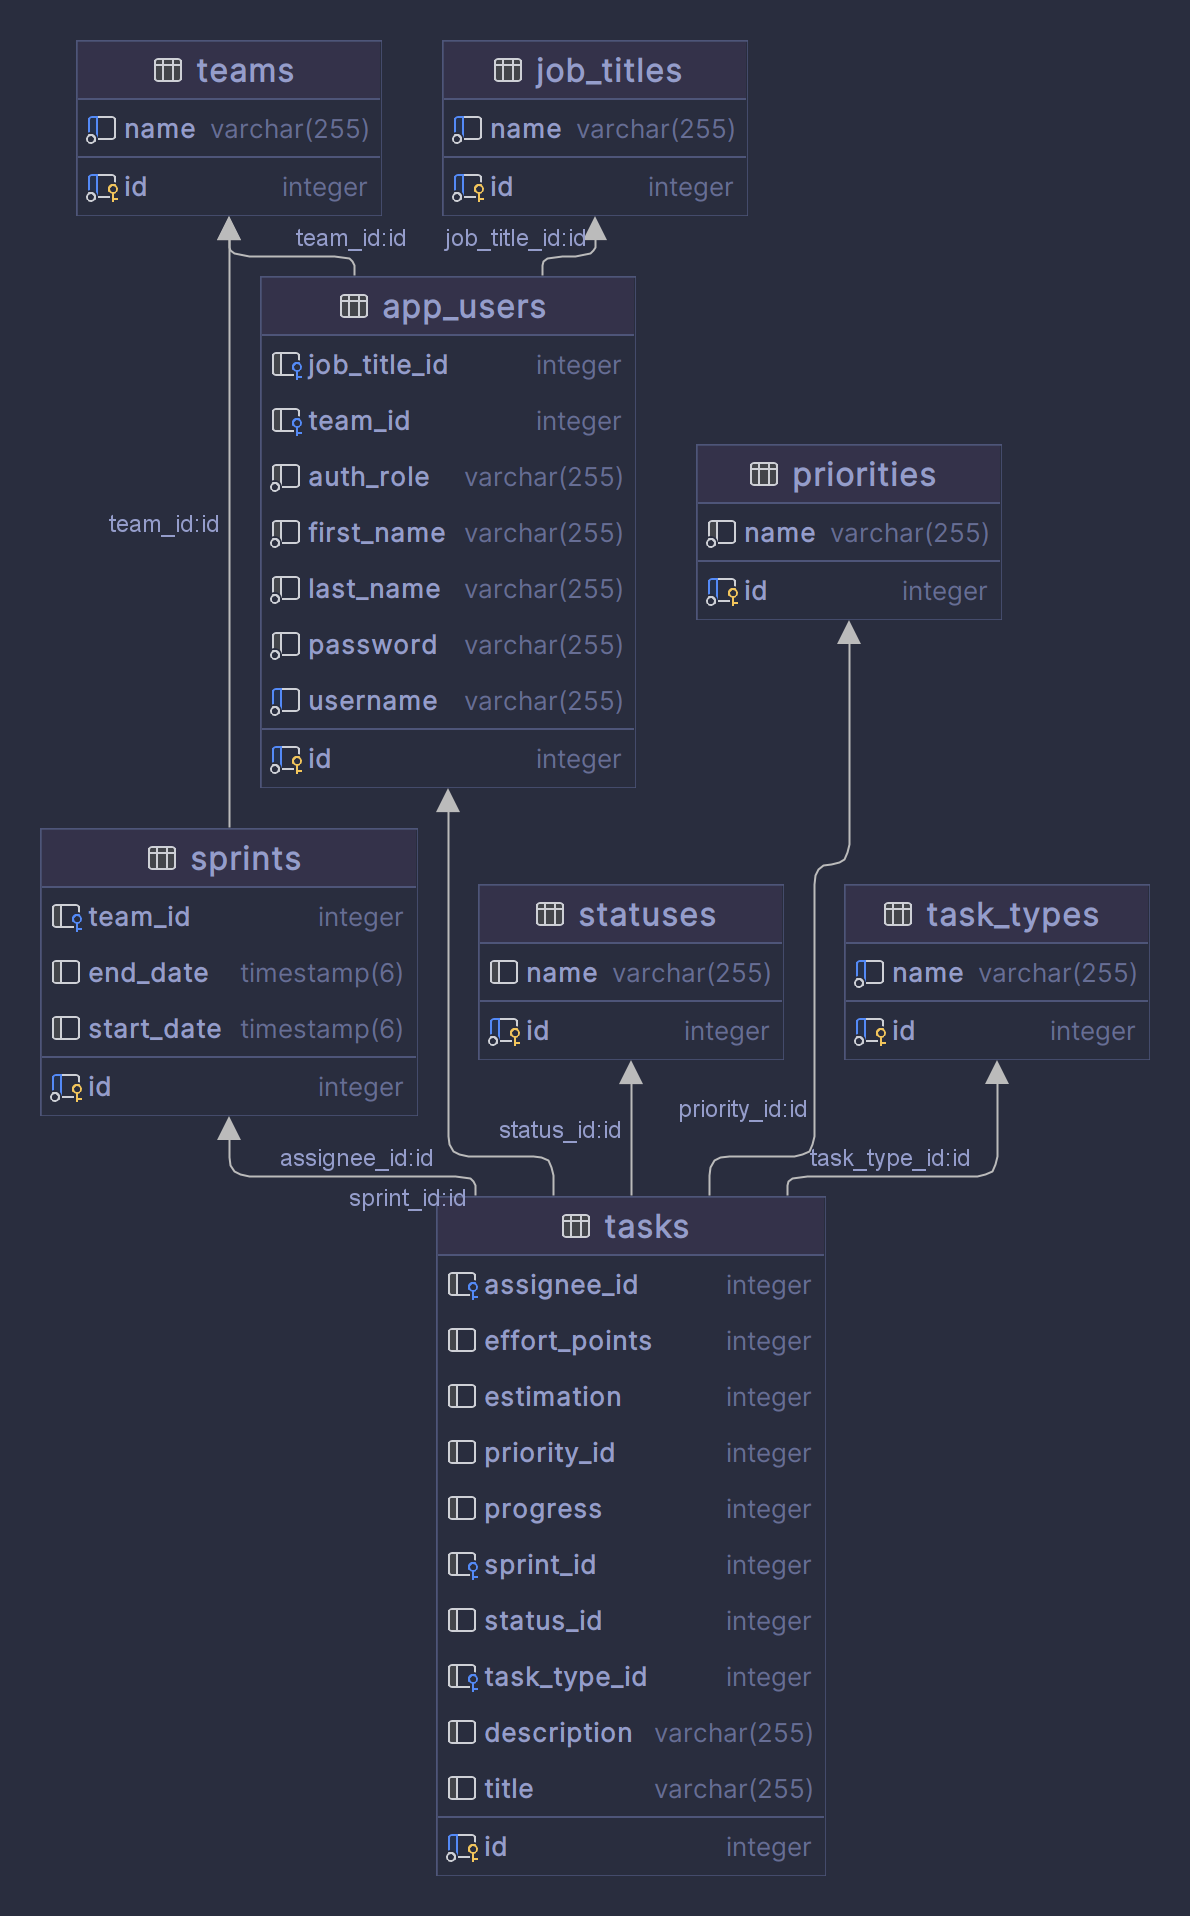
\includegraphics[width=0.7\linewidth]{taskage-db.png}
	\caption{Diagrama bazei de date}
	\label{taskage-db}
 \end{figure}

Nu numai interacțiunea cu baza de date este gestionată de Spring JPA, ci și schema acesteia, prin utilizarea unor configurări specifice. Astfel, fiecare clasă adnotată „@Entity” devine un tabel din diagrama 3.3, prin intermediul instrumentului de persistare a datelor Hibernate și al metadatelor oferite prin adnotări.

Tabela „app_users” are câmpul special „auth_role” care poate lua una din valorile „ROLE_BASIC”(asociat membrilor normali ai unei echipe), „ROLE_MANAGER”(asociat managerilor echipelor) și „ROLE_ADMIN”(asociat administratorului paginii), urmând formatul înțeles de Spring Security. Speciale mai sunt tabelele de tip dicționar „priorities” și „statuses”, care nu implementează operații CRUD, ci servesc la stocarea unor date care altfel ar fi fost stocate în structuri de tip enum. Această alegere ajută la organizarea eficientă a codului și permite manevrarea mai ușoară a valorilor, putând fi chiar și actualizate la runtime.

\section{taskage-client}

Componenta care constituie front-end-ul aplicației este taskage-client. Aceasta este un proiect React care folosește MobX pentru gestionarea stării. Una din provocările principale la construcția unui proiect în React este lipsa de structură interentă tehnologiei. Prin comparație cu un framework popular, Angular, proiectele React nu au o structură de fișiere și un flux de date bine-definite, acestea rămânând responsabilitatea dezvoltatorului. Cele două mari abordări pentru structurarea aplicației sunt: abordarea orientată pe cateogorie și abordarea orientată spre funcționalitate. Prima din cele două este mai puțin scalabilă, organizând fișierele după tipul lor(componente, pagini, modele, etc...) în timp ce a doua abordare rafinează mai departe structura, sortând componentele în funcție de funcționalitatea efectivă pe care o implementează. Am ales cea de-a doua alternativă pentru că densitatea componentelor devenise prea mare pentru a putea fi gestionate la un loc.

 \begin{figure}[ht]
	\centering
 	 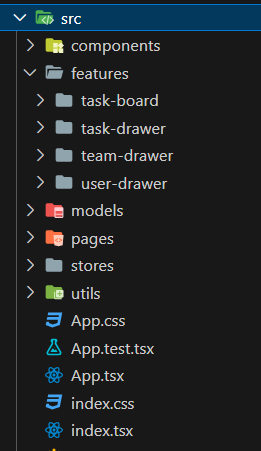
\includegraphics[width=0.3\linewidth]{FE-folder-structure.png}
	\caption{Structura de fișiere a aplicației React}
	\label{FE-folder-structure}
 \end{figure}

Deși front-end-ul reprezintă un SPA(Single Page Application), încărcarea paginilor se face pe baza rutelor pentru eficiență. Rutele sunt atât publice, cât și private. Cele private se pot accesa pe baza unor criterii precum tipul utilizatorului, iar în cazul lipsei privilegiilor de acces, acestea vor redirecționa utlizatorul către o pagină cu un mesaj sugestiv. Rutele servesc pagini, implementate în folderul „pages”, iar paginile randează diverse componente care, daca au logică complexă, sunt plasate într-un folder cu nume sugestiv funcționalității de care țin, în folderul „features”. Folderul „components” este rezervat pentru componente reutilizabile, generice.

Stocarea datelor necesare în componente aflate la distanță mare pe ierarhia din DOM se face in „stores”, concept specific MobX. Tot aici se fac si apelurile către server și gestionarea datelor utilizatorului spre setarea corespunzătoare a tokenului în header-ul cererilor.

\section{taskage-smart-helper}

[de adaugat capitol despre microserviciul pyhton dupa ce are o structura bine definita]